\chapter{Using Peptizer}
%
%
\npar This chapter explains the basics of using Peptizer. We will here explain how to \textbf{start a new Peptizer} task and how to \textbf{handle or save results} from such a task. Furthermore, we will indicate how to \textbf{distribute Peptizer data} and how to manage the \textbf{configuration files}.
%
%
\npar Once Peptizer has been set up as described in chapter \ref{installation}, start Peptizer by the \textit{peptizer.bat} (or \textit{peptizer.sh} in a UNIX environment) script. Upon launching the script, a window will appear from which Peptizer can be started (\ref{start_new_task}).
%
%Figure with the start up window
\begin{figure}[t!]
\begin{center}
	
\includegraphics[width=.85\textwidth]{start_new_task}
	\caption{\label{start_new_task}The start-up view of Peptizer. The top panel displays the menu bar wherein a new Peptizer Tasks can be started. The bottom panel displays a status panel with a welcoming message. The status panel will be updated upon user actions.}
\end{center}
\end{figure}
%
%Starting a task.
\section{Starting a Peptizer task}
%
%Pre word on  peptizer tasks
\npar Start a new task from the menu bar at the top (figure \ref{start_new_task}).
\npar Two types of tasks can be distinguished. The first and most important is \textbf{the selection task}. Here, the peptide hypothesises that were selected by the profile, are handled in the manual validation interface of Peptizer. A second task is \textbf{the ARFF task}. Here, the peptide hypothesises are handled into an ARFF file. This file contains all peptide hypothesises labelled whether they did or didn't match the profile along a feature vector with the Agent inspection results or votes.
%
%
%Subsection on a selection task
\subsection{Selection task}
\subsubsection{Overview}
\npar Start a new selection task by pressing \verb!Ctrl-T! or by \textit{clicking } in the menu bar at the top:
%
\begin{center}
\textit{Main // New Task // Selection Task}	
\end{center}
%
%
\npar A new dialog appears wherein a new task can be created(\ref{new_selection_task_coded}). \\Therein, the important parts of the dialog are labelled by characters. Just below the figure, a short explanation is shown.
%
\pagebreak
%FIGURE with the selection task coded overview.
\begin{figure}[H]
\begin{center}
	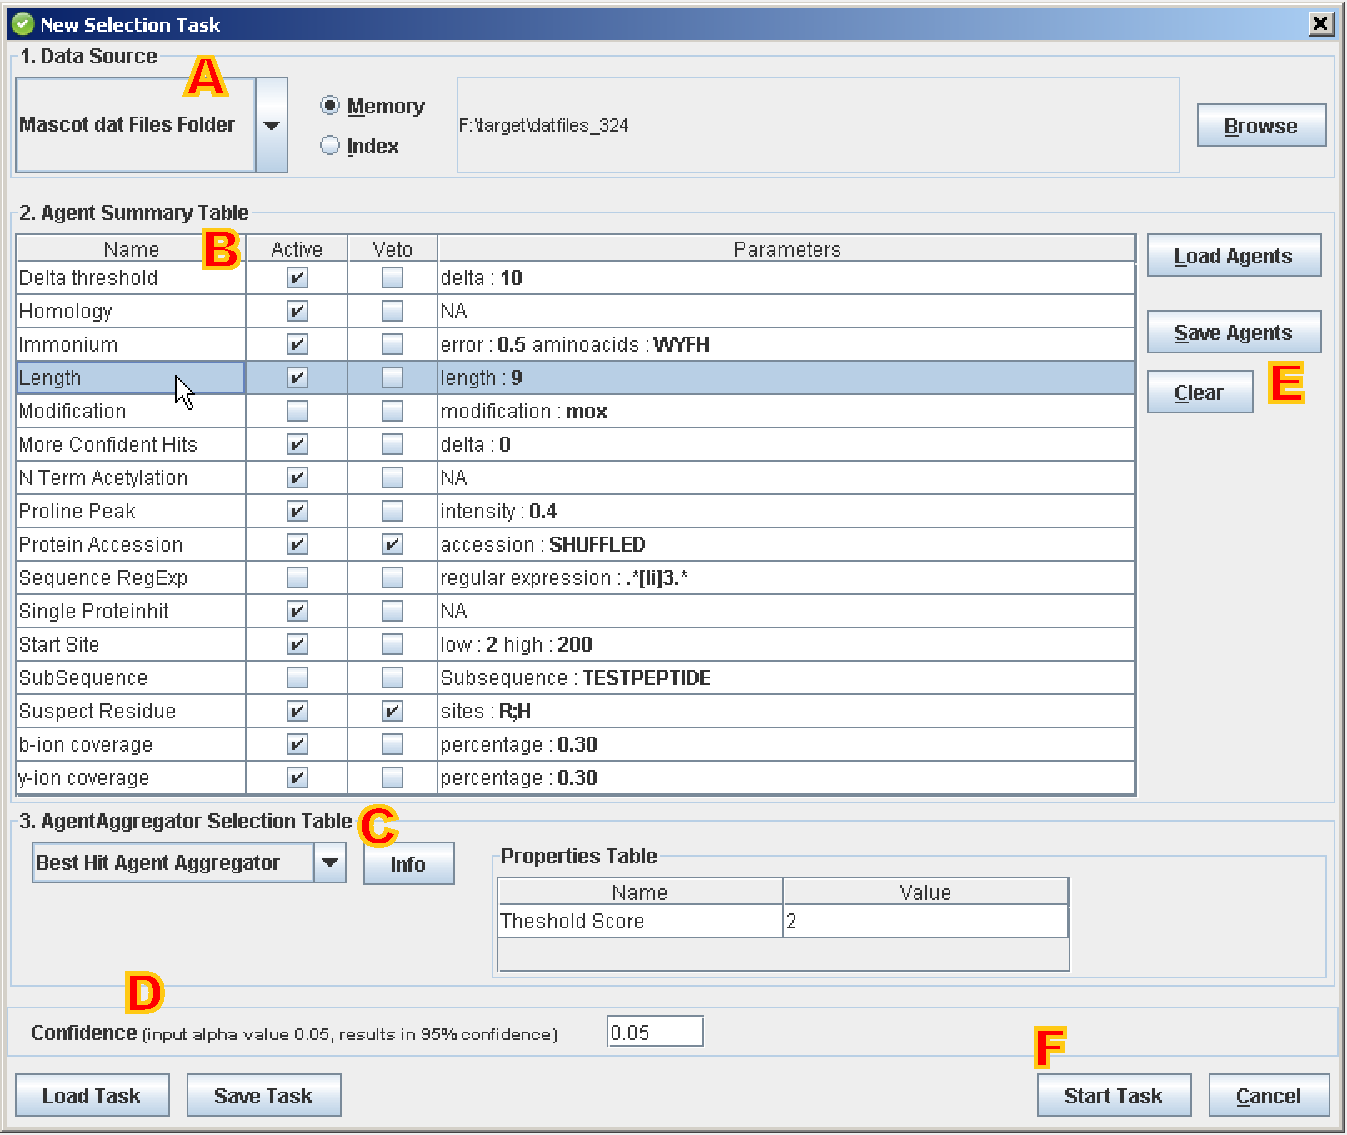
\includegraphics[width=.85\textwidth]{new_selection_task_coded}
	\caption{\label{new_selection_task_coded} Overview of the new selection task dialog. The data source is defined in A. The Agents are activated and customized in B. The AgentAggregator is selected and customized in C. The Mascot confidence level for peptide hypothesises is defined in D. Agent configuration files can be cleared, stored or loaded in E and, finally, a new task can be started in F.}
\end{center}
\end{figure}
%
%LIST with figure codings.
\renewcommand{\labelenumi}{\Alph{enumi}.}
\begin{enumerate}
	\item Defining the data source.\\\textit{Which MS/MS spectrum identifications must be processed?}
	\item Activating and customizing Agents.\\\textit{What rules do the peptide identifications have to fit?}
	\item Selecting and customizing the AgentAggregator.\\\textit{How should the Agent votes be aggregated to judge a peptide hypothesis?}
	\item Defining the Mascot probability.\\\textit{When is a peptide hypothesis considered confident?}
	\item Storing, clearing or loading a Peptizer configuration.\\\textit{What pre-defined configuration must be used?}
	\item \textit{Start the selection task!}
\end{enumerate}
\npar Each of these parts are explained into more detail below.
%
%SUBSECTION ON DATA SOURCE
%
\subsubsection{Defining the data source}
%
\npar The data source relates to the peptide hypothesises that must be inspected. Peptizer currently only inspects peptide hypothesises from Mascot result files. These files are stored at the Mascot server and contain the core results of the interpreted MS/MS data. Different data sources can be defined in Peptizer from the pull-down menu.
\begin{description}
	\item[Mascot dat Files Folder ] Select a folder using the \textit{browse} button. Peptizer will then process all the peptide hypothesises in all Mascot result files in that selected folder (other files in that folder will be ignored).
	\item[Mascot dat File ] Select a Mascot result file by the \textit{browse} button. Peptizer will then process all the peptide hypothesises in the selected Mascot result file.
	\item[ms\_lims project] Create a ms\_lims database connection using the \textit{create connection} button.\footnote{ms\_lims stands for Mass Spectrometry oriented LIMS system (more information can be found at \url{http://genesis.ugent.be/ms_lims/}), which organizes raw MS/MS data and their interpretation by Mascot in a project-wise fashion.} Once a connection is established, select a ms\_lims project from the pull-down menu. Peptizer will then process all the peptide hypothesises in the ms\_lims project.
	\item[ms\_lims identification id] After a connection to a ms\_lims database has been established, enter one ms\_lims identification id per line in the textarea. Peptizer will then process only the MS/MS spectra and their peptide hypothesis of the given identification ids.
\end{description}
\npar The Mascot result files can be parsed in two different ways. Select the appropriate radio button:
\begin{description}
	\item[Memory] uses in-memory parsing. This is fastest though very memory intensive.\\Use this option for files up to tens of megabytes.
	\item[Index] uses index-based parsing. This is slower however far less greedy on virtual memory.\\Use this option for files above 100MB.
\end{description}

%
%SUBSUBSECTION ON AGENTS
%
\subsubsection{\label{agentpanel}Activating and customizing the Agents}
\npar Each Agent inspects a property of a peptide hypothesis and casts a vote on each element coming from the data source. This vote has either an approving, reserving of rejecting opinion for the final grouping of peptide hypothesises. This table serves to select one or more Agents altogether having the properties of the peptide hypothesises that will be merged.
\npar Each table row represents an Agent and each table column relates to another function in Peptizer:
\begin{description}
	\item[Name] Very short identifier of an Agent serving as a row header.
	\item[Active] Simple conditional whether this Agent should be used or not. Check this checkbox if an Agents inspection must be enabled. 
	\item[Veto] Extra rights for an Agent vote. If checked, a peptide hypothesis will always be selected when this Agent approves selection. 
	\item[Parameters] Optional settings for an Agent. Some Agents require an additional parameter, this is mostly a user-defined threshold used by the Agent during inspection. If the parameter says 'NA', no parameters are to be set. Else, the table shows the current settings. These can be modified by \textit{double-clicking} the parameters.
\end{description}
%
\begin{center}
	\fbox{
        	 \begin{minipage}[t]{1.0\textwidth}
	            \textsc{Hint}\\A short tooltip describing an Agents logic can be shown by \textit{holding} the mouse cursor on its name cell.
        	 \end{minipage}
         }
\end{center}
%
%SUBSUBSECTION ON AGENTAGGREGATORS
%
\subsubsection{Selecting and customizing the AgentAggregator}
\npar The AgentAggregator aggregates the votes from the different Agents. As there are different logical paths for aggregation, there are different AgentAggregators. Select an appropriate AgentAggregator by \textit{clicking} the pull-down menu on the left. By \textit{clicking} the info button a dialog will pop up describing the selected AgentAggregator. This dialog informs on the general concept, the logic of the aggregation and the optional settings. An example dialog for the BestHitAgentAggregator is shown in figure \ref{besthitagentaggregator_description_dialog}.\footnote{As we cannot document custom built AgentAggregators in this manual, we opted for documentation by the configuration files that can also be viewed in real-time. We therefore refer to Peptizer for documentation on the different types of AgentAggregators.} Modify these optional settings by \textit{double-clicking} the value cells.
%%%%%%%
%FIGURE%
%%%%%%%
\begin{figure}[t!]
\begin{center}
	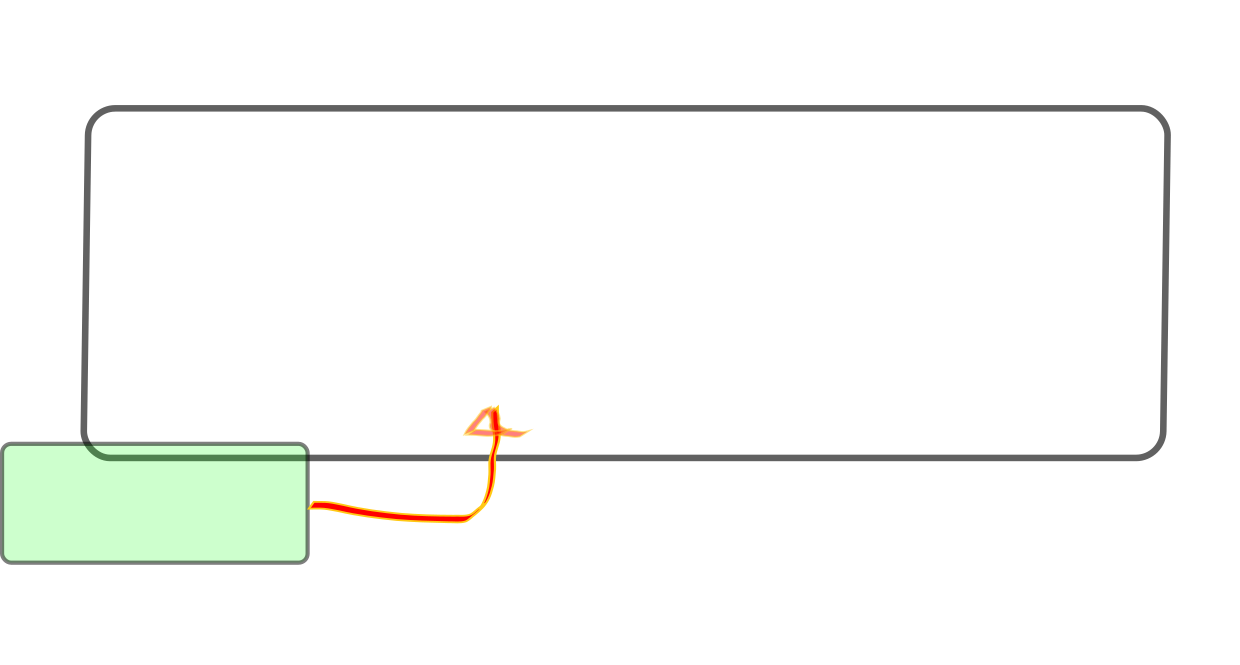
\includegraphics[width=.85\textwidth]{besthitagentaggregator_description_dialog}
	\caption{\label{besthitagentaggregator_description_dialog} The AgentAggregator information dialog. By clicking the info button, a description dialog informs on the general concept, the logic of the aggregation and the optional settings of the selected AgentAggregator.}
\end{center}
\end{figure}
%
%SUBSUBSECTION ON CONFIDENCE
%
\subsubsection{Defining the Mascot confidence}
\npar The Mascot Identity Threshold (MIT) is calculated for a given alpha value. This alpha value reflects the probability that a peptide hypothesis is random.\\Insert an appropriate alpha value for MIT calculation in the textfield at the bottom. Only peptide hypothesises with a Mascot Ion Score (MIS) higher then the MIT will be considered by Peptizer. Note that secondary and tertiary ranked peptide hypothesises with a MIS $>$ MIT will be considered by Peptizer.
%
%SUBSUBSECTION ON CONFIGURATION FILES
%
\subsubsection{Storing, clearing or loading a Peptizer configuration}
\npar Once a set of Agents is selected and customized, that configuration can be saved into an Agent configuration file. These files can be re-loaded at a future time or at another place. Save or load an Agent configuration file by \textit{clicking} the Save Agents button (\verb!Alt-S!) or the Load Agents button (\verb!Alt-L!). By \textit{clicking} the clear button (\verb!Alt-C!), the table will be reset for a clean start.
\par Find out more on the configuration files in section \ref{configuration_files}.
%
%
%
%SUBSECTION ON ARFF TASK
\subsection{ARFF task}
%QUOTATION FROM WEKA
\begin{quote}
  \textsf{"An ARFF (Attribute-Relation File Format) file is an ASCII text file that describes a list of instances sharing a set of attributes. ARFF files were developed by the Machine Learning Project at the Department of Computer Science of The University of Waikato for use with the Weka machine learning software."}\\Quotation from \url{http://www.cs.waikato.ac.nz/~ml/weka/arff.html}.
 \end{quote}
\npar The Arff task is similar to the Selection Task as Agents and AgentAggregators are similarly selected and customized. The difference lies in the output presentation to the user. Instead of presenting the selected peptide hypothesises in the manual validation interface, a single ARFF file is produced containing all the peptide hypothesises. For each peptide hypothesis, Peptizer creates a feature vector and a single label. One feature relates to one Agent inspection and the label corresponds with the aggregation result.
\subsubsection{Overview}
\npar Start a new Arff task by by pressing \verb!Ctrl-A! or by \textit{clicking }the menu bar in the top:
%
\begin{center}
\textit{Main // New Task // Arff Task}	
\end{center}
\npar In the Arff Task dialog two types of information can be chosen to fill the feature vector. Choose by \textit{clicking} on one of the following radio buttons:
\begin{description}
	\item[Detailed result] The feature is the peptide hypothesis variable used upon inspection.\\e.g. \textit{'6' will be the feature value upon inspection of a 6 amino acid long peptide by the Length Agent requiring a peptide hypothesis to be longer then 8 amino acids.}
	\item[Match result] The feature value is the Agent vote after inspection.\\e.g. \textit{'1' will be the feature value upon inspection of a 6 amino acid long peptide by the Length Agent requiring a peptide hypothesis to be longer then 8 amino acids.}
\end{description}
%
\npar The main purpose of this task type is to show that different tasks can be created with the common concept of Agents and AgentAggregators. Peptizer itself is focussed at the level of a single peptide hypothesis. Therefore, we directed this task specifically towards more advanced data-analysis at the level of groups of peptide hypothesises.
\npar Besides the WEKA library, Arff files produced by Peptizer can be interpreted by free initiatives such as \textbf{Rapidminer}\footnote{RapidMiner is an open-source data mining solution combining both leading-edge technologies and a broad functional range. Applications of Rapidminer cover a wide range of real-world data mining tasks.\\More information on the Rapidminer community edition can be found at \\\url{http://rapid-i.com/content/blogcategory/10/69/lang,en/}} or the \textbf{R/Weka package} for the R\footnote{R is a free software environment for statistical computing and graphics.\\More information on R can be found at \url{http://www.r-project.org/}} project of statistical computing.

%
%SECTION ON HANDLING A PEPTIZER TASK
\section{Handling a Peptizer task}
\npar As manual validation is a tricky and time-consuming job, this should be facilitated as much as possible. First, the user only validates those peptide hypothesises selected by set criteria. As such, no time is spend on peptide hypothesises that are not of interest. Second, the user is placed in an \textbf{optimal environment} to make a final decision on the validity of a peptide hypothesis. In such an environment, the user has a compact view with \textbf{general information }and \textbf{spectral information }along with \textbf{Agent-driven pluggable information}. These are core ideas of the Peptizer platform, both assisting the manual validation process and improving the specificity of the results.
\npar After a selection task is finished, the selected peptide hypothesises are shown in the manual validation interface of Peptizer. The following section explains how to handle the task results in Peptizer's manual validation interface.

\subsection{Overview}
\npar The main functions of the manual validation interface of Peptizer are shown in figure \ref{validation_GUI}.
\npar The peptide hypothesises selected by the criteria defined by Agents and AgentAggregators are listed in the \textbf{Identification Tree}. The tree header displays the size and the overall validation status. Each spectrum node in the tree is an identified MS/MS spectrum and unfolds peptide hypothesises from this MS/MS spectrum as tree leaves. Also, the tree can be filtered by validation status or by Agent vote.
\npar By \textit{double-clicking} a spectrum node, a new \textbf{MS/MS spectrum identification} tab is added into the central panel. Therein, the suggested peptide sequence and MS/MS spectrum annotated by fragmentation information is presented. In the bottom of a MS/MS spectrum identification tab an information table is shown with both general and Agent information are shown. The MS/MS spectrum identification can be validated by the buttons on the bottom right edge.
\npar Finally, in the very bottom, the \textbf{Status Pane} logs actions performed in Peptizer.
%%%%%%%%%%%%%%%%%%%%%
%FIGURE WITH MAIN FUNCTIONS%
%%%%%%%%%%%%%%%%%%%%%
\begin{figure}
\begin{center}
	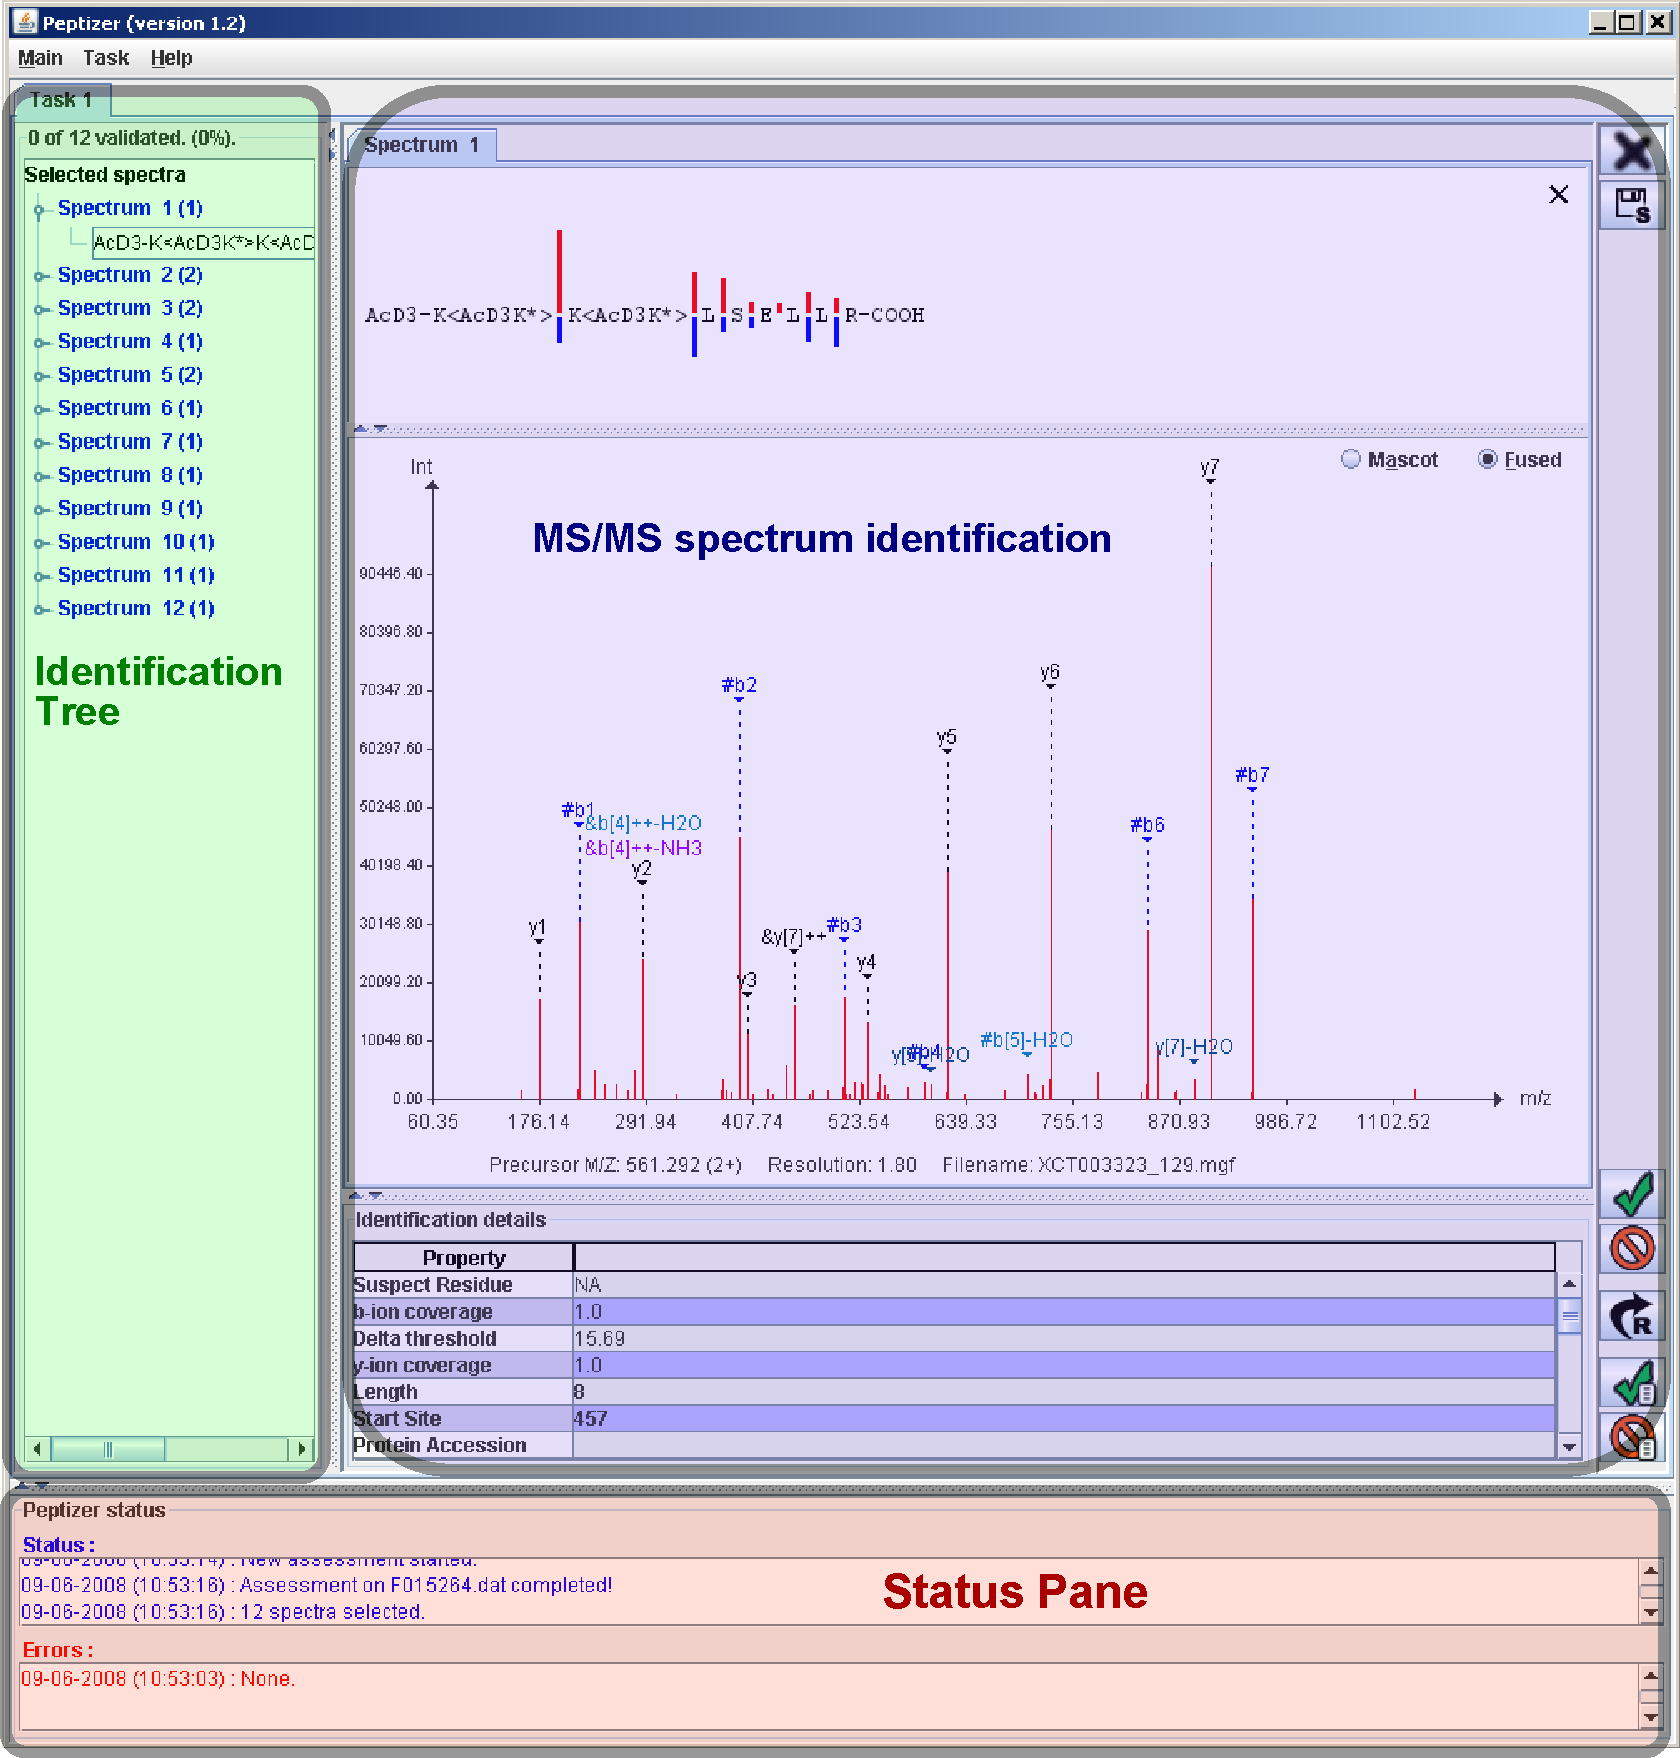
\includegraphics[width=.8\textwidth]{validation_GUI}
	\caption{\label{validation_GUI}An overview of the main functions of the Peptizer validation gui. On the left side is the Identification Tree with the selected MS/MS spectra. By double clicking a spectrum tree node, a MS/MS spectrum identification tab of that spectrum is added in the central panel. In the bottom, the Status Pane is updated upon a variety of actions.}
\end{center}
\end{figure}
%
\pagebreak
\subsection{Identification tree}
The identification tree is shown in figure \ref{identification_tree}
%%%%%%%%%%%%%%%%%%%%%%%%
%FIGURE WITH IDENTIFICATION TREE%
%%%%%%%%%%%%%%%%%%%%%%%%
\begin{figure}[t!]
\begin{center}
	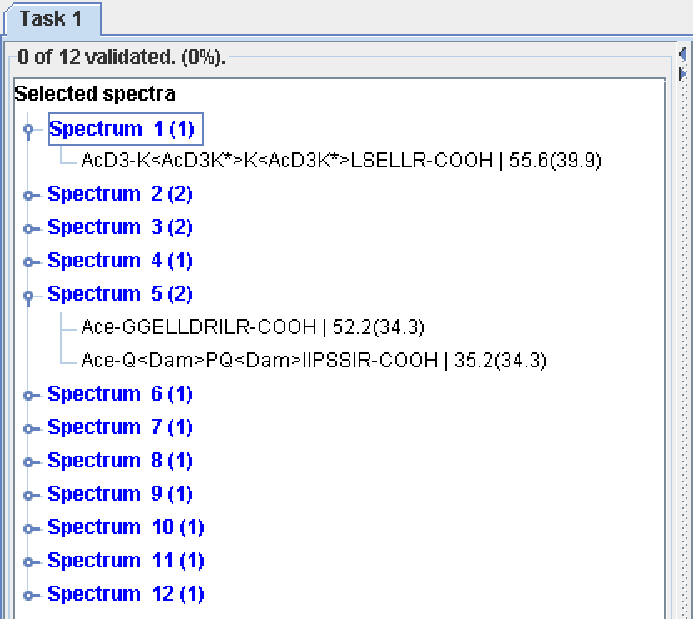
\includegraphics[width=.6\textwidth]{identification_tree}
	\caption{\label{identification_tree}The Identification Tree lists the selected MS/MS spectra. The tree header displays the size and the validation status. The tree unfolds first with spectrum nodes and then with peptide hypothesis nodes. By \textit{double-clicking }the spectrum node, its peptide hypothesises are presented in detail in another panel.}
\end{center}
\end{figure}
%
\npar The Identification Tree header displays a number summary of the validation status. In figure \ref{identification_tree}, the header \verb!"O of 12 validated. (0%)"! means that none of the 12 selected MS/MS spectra was validated. Each of these 12 spectra are presented as spectrum nodes. By \textit{double-clicking }a spectrum node, a new MS/MS spectrum identification tab is added in the center panel (see \ref{peptide_identification_tab}). Such a spectrum node has the folowing structure:\begin{verbatim}Spectrum list identifier (Number of confident peptide hypothesises)\end{verbatim}
The spectrum node displays the number of confident peptide hypothesises, which reside as tree leaves beyond each spectrum node. For example \verb!"Spectrum 5 (2)"! in figure \ref{identification_tree} indicates that there were 2 confident peptide hypothesises for MS/MS spectrum 5. Such a peptide hypothesis leaf has the following structure:\begin{verbatim}Modified peptide sequence | Mascot Ionscore (Mascot Identity Threshold)\end{verbatim}
\npar Upon validating a MS/MS spectrum, the spectrum node colours green or red when respectively accepting or rejecting the spectrum node. Also note that the tree header updates the validation status.
\npar A filter can be applied on the Identification Tree, which facilitates navigation through larger trees.
\npar Apply a filter by \textit{clicking }the menu bar in the top:
%
\begin{center}
\textit{Task // Filter // ...}	
\end{center}
\npar Disable one or both filters by \textit{clicking }the menu bar in the top:
%
\begin{center}
\textit{Task // Filter // Disable filters}	
\end{center}
\npar The effect of two different filters is shown in figure \ref{identification_tree_filter}.
%
%%%%%%%%%%%%%%%%%%%%%%%%%%%%%
%FIGURE WITH  TREE FILTER   %
%%%%%%%%%%%%%%%%%%%%%%%%%%%%%
%
\begin{figure}[t!]
\begin{center}
	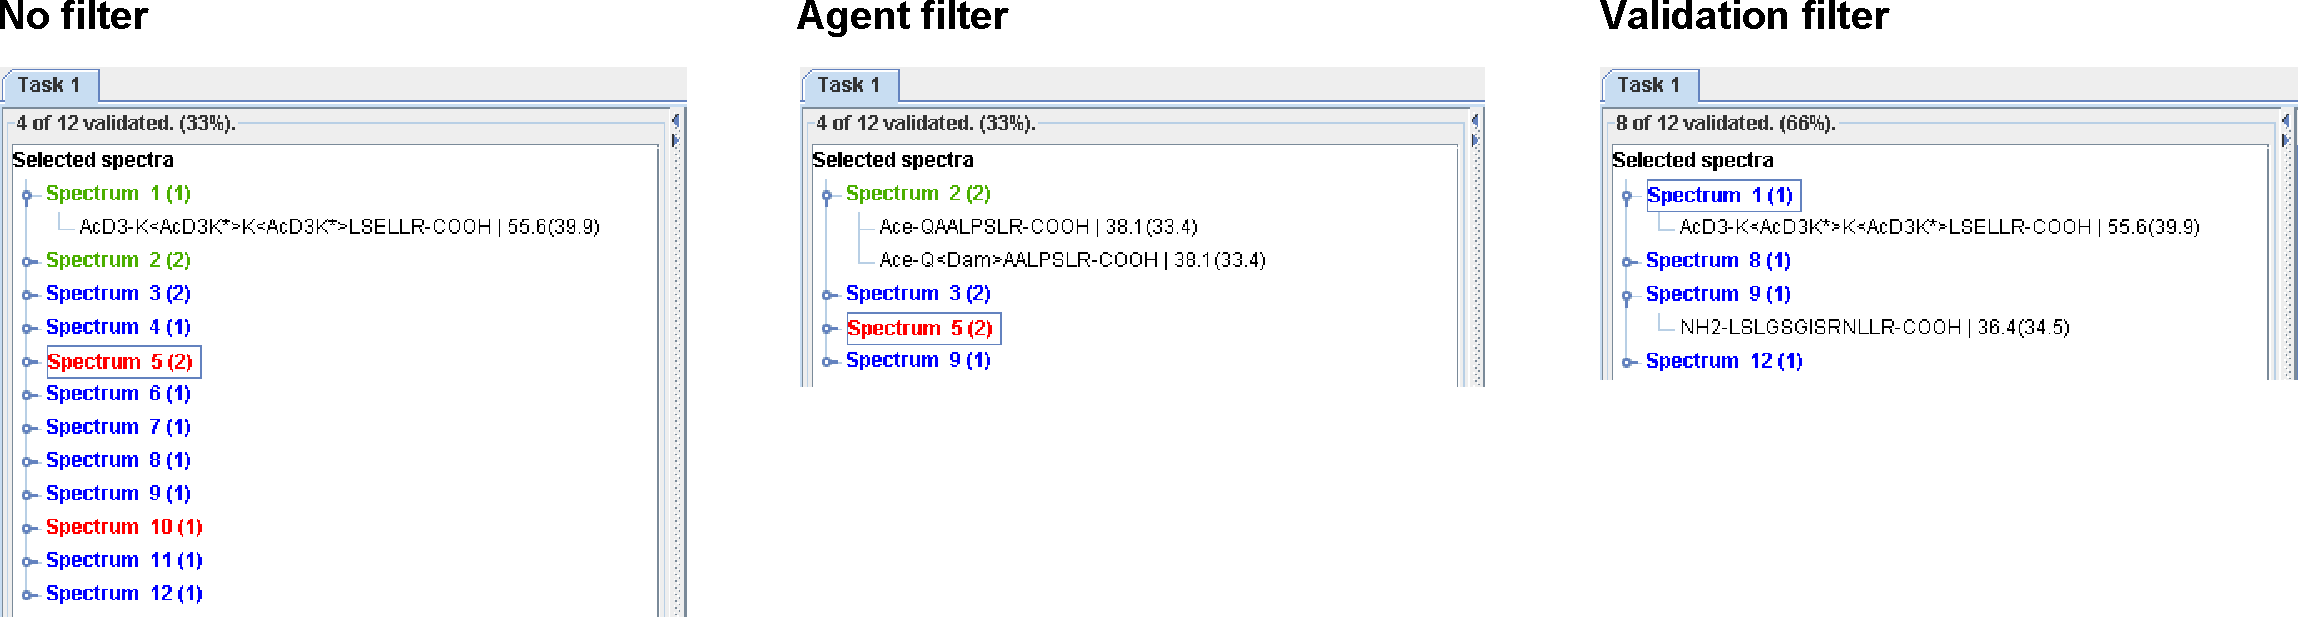
\includegraphics[width=.95\textwidth]{identification_tree_filter}
	\caption{\label{identification_tree_filter}The Identification Tree filters. On the left, no filters are applied. In the middle, the Agent filter was applied and therefore only the MS/MS spectrum identifications with a selective vote for that Agent are shown. On the right, the validation filter was applied and therefore all validated MS/MS spectrum identifications are now hidden.}
\end{center}
\end{figure}
%
%%%%%%%%%%%%%%%%%%
%DESCRIPTION OF FILTERS%
%%%%%%%%%%%%%%%%%%
\begin{description}
	\item[Agent filter] shows MS/MS spectrum identifications by  Agent votes.
	\item[Validation filter] shows MS/MS spectrum identifications that have not been validated yet.
\end{description}
%%
\newpage
\subsection{\label{peptide_identification_tab}MS/MS spectrum identification tab}
\npar The central panel displays multiple tabs. Each tab is a MS/MS spectrum identification tab showing all details on one MS/MS spectrum and its proposed peptide hypothesis(es). These peptide hypothesises are theoretically fragmented by Peptizer to align them with the MS/MS spectrum. This yields\textbf{ fragmentation information} that is combined with \textbf{general information}. The MS/MS spectrum identification tab also shows \textbf{pluggable information} driven by Agent inspections. Finally, an MS/MS spectrum identification can be validated here.
\npar These different types of information are illustrated below(figure \ref{Peptide_Identification_info}).
\npar A MS/MS spectrum identification can be closed in the pop-up menu by \textit{right-clicking }the tab or by \textit{clicking} the small 'x' button on the top-right. All spectrum tabs can be cleared by \textit{clicking} the large 'X' on the top-right.
%
%%%%%%%%%%%%%%%%%%%%%%%%%%%%%
%FIGURE WITH  PEPTIDE IDENTIFICATION TAB %
%%%%%%%%%%%%%%%%%%%%%%%%%%%%%
%
\begin{figure}[h!]
\begin{center}
	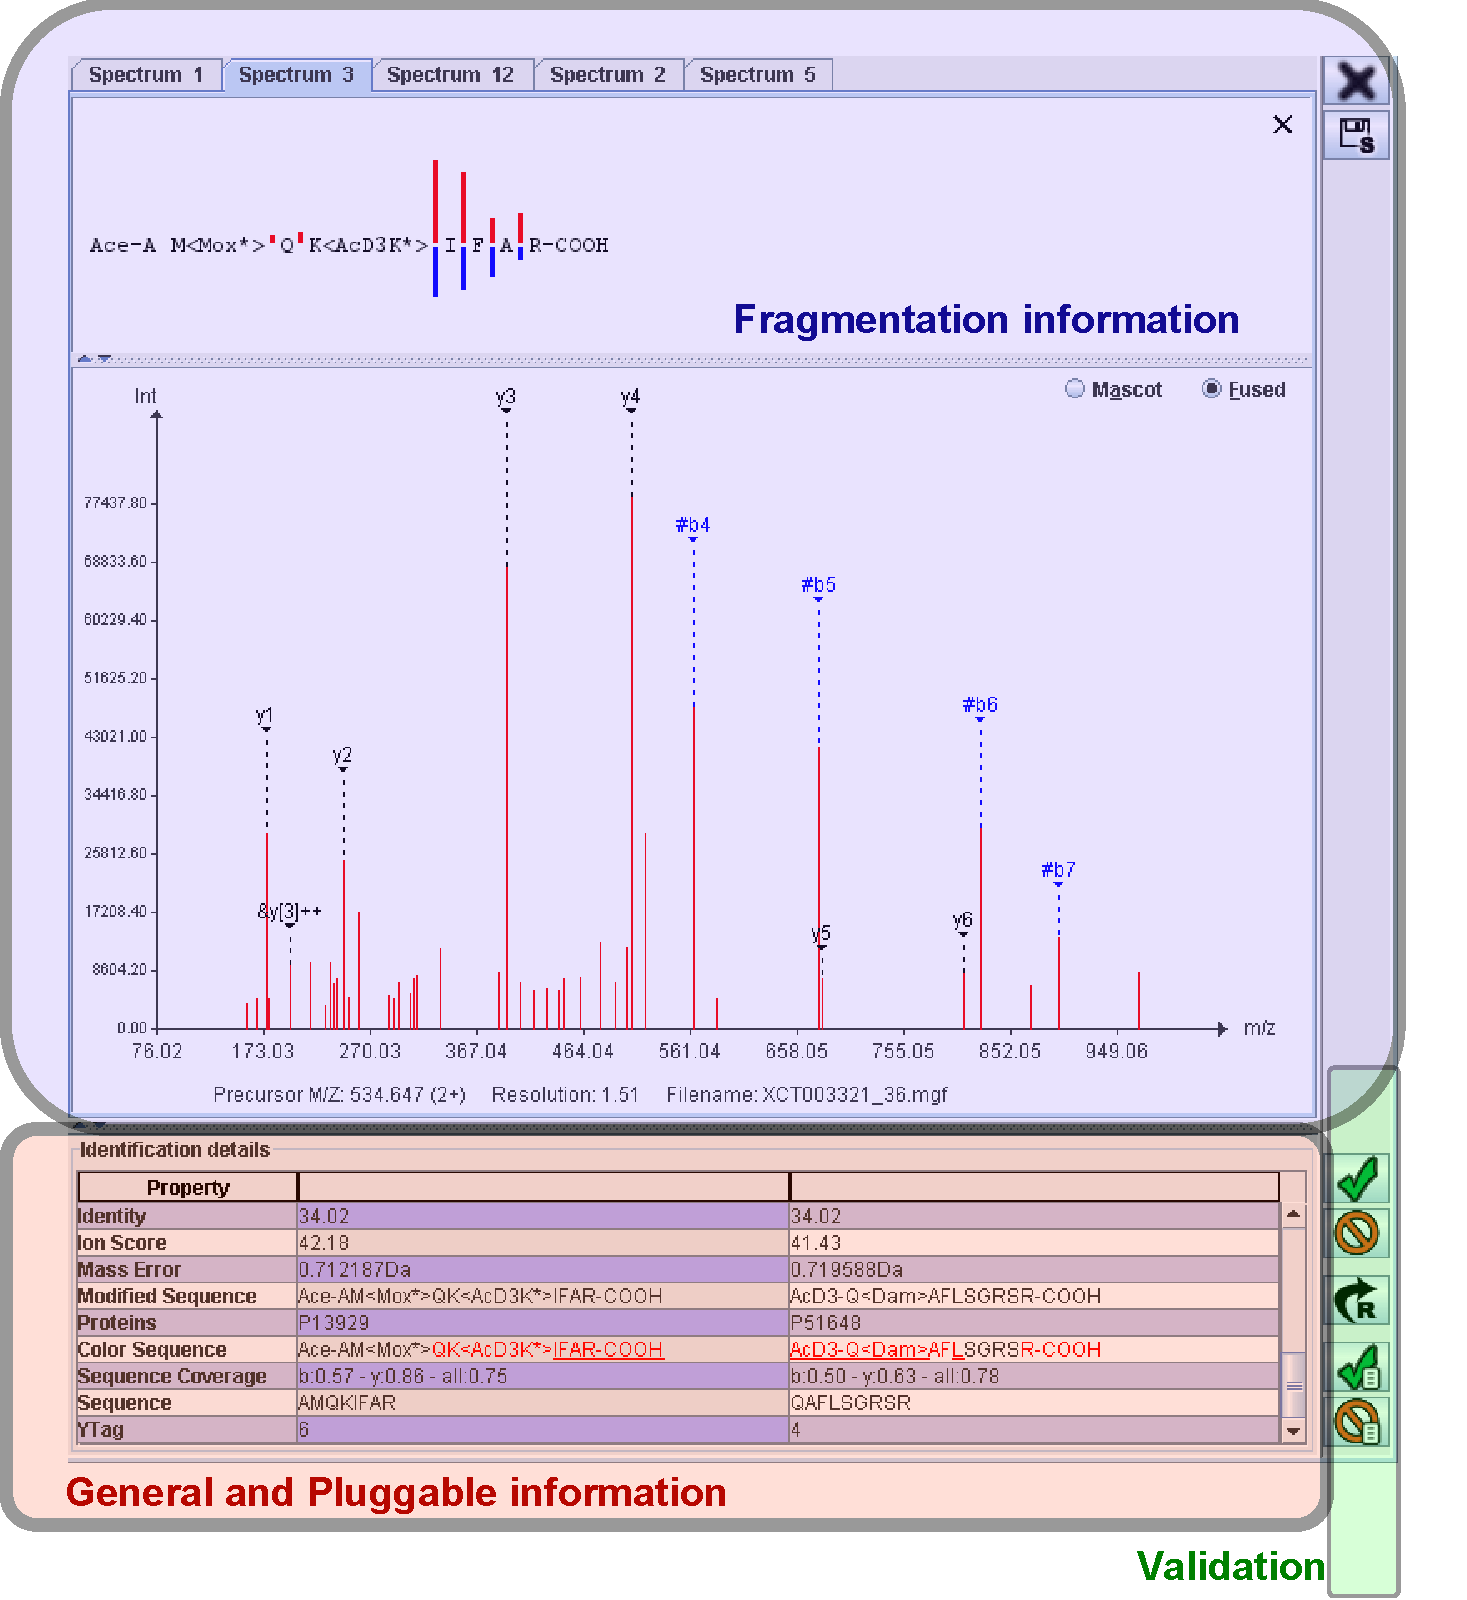
\includegraphics[width=.90\textwidth]{Peptide_Identification_info}
	\caption{\label{Peptide_Identification_info} Each MS/MS spectrum identification tab displays information on a single MS/MS spectrum and its confident peptide hypothesis(es). In this tab, Peptizer combines fragmentation, general and pluggable information along with validations.}
\end{center}
\end{figure}
%
\subsubsection{Fragmentation information: The annotated MS/MS spectrum}
\npar The MS/MS spectrum is stored in the Mascot result files. This is used to draw the MS/MS spectrum on a custom Spectrumpanel component. The X-axis and Y-axis respectively plot the mass over charge and intensity values of the fragment ions. The user can interpret the fragmentation spectrum by the following actions:
%%%%%%%%%%%%%%%%%%%%%%%%%%%%%%%%%%%%%
%DESCRIPTION OF DIFFERENT SPECTRUMPANEL ACTIONS%
%%%%%%%%%%%%%%%%%%%%%%%%%%%%%%%%%%%%%
\begin{description}
	\item[Left click in the spectrum ]and drag a mass over charge interval to zoom into that range.
	\item[Right click ] zooms out to the complete MS/MS spectrum.
	\item[Hoovering] the cursor over a peak shows the mass over charge value for that peak.
	\item[Left click on a peak] starts peak-picking. If the cursor is moved on top of another peak, the mass over charge difference of those peaks is shown. By clicking another peak, this difference in mass is fixed and peak picking can be continued. Note that if this mass difference corresponds to an amino acid or a modified amino acid, the mass difference is annotated by that component.
	\item[Ctrl + Left click] resets the primary peak picking.
	\item[Alt + Left click] holds the primary peak picking in a red font and starts a secondary peak-picking.
\end{description}
%
\npar As Peptizer simulates the theoretical fragmentation of the peptide hypothesis, it can annotate MS/MS spectra.
\npar For better understanding, the Mascot "\textbf{ionseries}" variable must first be explained. Mascot scores a peptide hypothesis for a MS/MS spectrum by the evidence found for a specific type of fragment ions. Two different types of fragment ions can for example be b-ions and y-ions, while double charged b++-ions and y++-ions are two other types. The different types of fragment ions are listed in the table below.
% Table generated by Excel2LaTeX from sheet 'Sheet1'
\begin{center}
\begin{tabular}{rl}
{\bf Ion Type} & {\bf Neutral Mr} \\

        a  & [N]+[M]-CHO \\

       a*  &      a-NH$_3$ \\

       a�  &      a-H$_2$O \\

        b  &  [N]+[M]-H \\

       b*  &      b-NH$_3$ \\

       b�  &      b-H$_2$O \\

        c  & [N]+[M]+NH$_2$ \\

        d  & a - partial side chain \\

        v  & y - complete side chain \\

        w  & z - partial side chain \\

        x  & [C]+[M]+CO-H \\

        y  &  [C]+[M]+H \\

       y*  &      y-NH$_3$ \\

       y�  &      y-H$_2$O \\

        z  & [C]+[M]-NH$_2$ \\
\end{tabular}  
\end{center}

\npar The fragment ion masses can be calculated when [N] is the molecular mass of the neutral N-terminal group, [C] is the molecular mass of the neutral C-terminal group and [M] is molecular mass of the neutral amino acid residues.\footnote{More information on the different types of ionseries can be found on-line at the Mascot help pages. \url{http://www.matrixscience.com/help/fragmentation_help.html}}
\npar The ionseries variable comes with each peptide hypothesis and lists the ion types that Mascot considered relevant to propose this peptide hypothesis. Opposite to the Mascot HTML result page, this valuable information is used when annotating the MS/MS spectrum. This is illustrated by an annotated MS/MS spectrum shown in figure \ref{annotated_MSMSspectrum}.
%%%%%%
%FIGURE%
%%%%%%
\begin{figure}[t!]
\begin{center}
	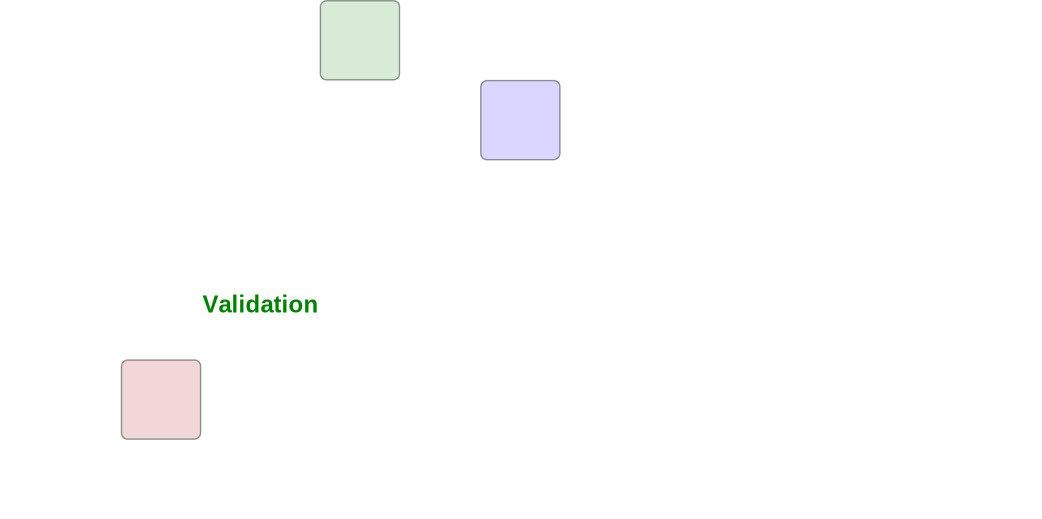
\includegraphics[width=.85\textwidth]{annotated_MSMSspectrum}
	\caption{\label{annotated_MSMSspectrum}The MS/MS spectrum annotated by relevant fragment ion types.}
\end{center}
\end{figure}
\npar The relevance of the ion type is encoded by the prefix:
\begin{description}
	\item[plain y3] means that Mascot found y-ions significant and used these to score the peptide hypothesis.
	\item[hash \#b4] means that Mascot found b-ions significant, however they were not used to score the peptide hypothesis.
	\item[ampercent \&y++3] means that Mascot found double charged y-ions not significant and they were not used to score the peptide hypothesis.
\end{description}
\npar Finally, the Mascot and Fused annotation types can now also be explained.\label{annotationtypes}
\begin{description}
	\item[Mascot annotations] show those fragment ion types significant for Mascot. Moreover, only the most relevant peaks are annotated.\footnote{The most relevant peaks by the Mascot annotation are defined by the PeaksUsedFromIons1 variable of a peptide hypothesis. This is the number of peaks that were used to propose the peptide hypothesis.}
	\item[Fused annotation] show the Mascot annotations plus immonium ions and the non-significant ion types (those prefixed with '\&'). Also, all peaks are annotated if they are more intense then 10\% of the most intense peak. 
\end{description}
\npar Swap between both types by clicking the corresponding radio button at the top of the panel.
\npar As such, one can briefly inspect the MS/MS spectrum and its peptide hypothesises, as suggested by Mascot and supplemented with additionla fragment ion data.
%
\subsubsection{Fragmentation information: The annotated peptide sequence}
\npar After simulating the theoretical fragmentation of the peptide hypothesis, Peptizer aligns this fragmentation information with the peptide sequence. This type of presentation was inspired by GPMDB.\footnote{The Global Proteome Machine Database was constructed to utilize the information obtained by GPM servers to aid in the difficult process of validating MS/MS spectrum identifications as well as protein coverage patterns. \url{http://gpmdb.thegpm.org/}}
\npar An illustration of an annotated sequence is shown in figure \ref{annotated_peptide_sequence}.
%
%%%%%%
%FIGURE%
%%%%%%
\begin{figure}[h!]
\begin{center}
	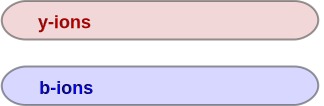
\includegraphics[width=.6\textwidth]{annotated_peptide_sequence}
	\caption{\label{annotated_peptide_sequence}The peptide sequence annotated by b and y fragment ions.}
\end{center}
\end{figure}
%
\npar The image is interpreted as follows. If the peptide bond fragmented and led to a b or b++ ion, a blue bar is shown below that peptide bond. Else, if the peptide bond fragmented and lead to a y or y++ ion, a red bar is shown above that peptide bond. All bars are relative to the peak intensity, where the most intense annotated peak in the MS/MS spectrum is set as the maximum bar.
%
\npar The fragmentation annotation on the MS/MS spectrum and the peptide sequence are complementary. This is illustrated in figure \ref{annotated_combining}. Here, the y1 and b7 ion are each on one side of the MS/MS spectrum, they do however originate from fragmentation of the same peptide bond. This cannot easily be seen in the annotated MS/MS spectrum since it is based on mass over charge values. Moreover, in this example, the annotated sequence shows that the C-terminal end of the peptide fragmented well and further indicates which peptide bonds broke most efficiently. Still, the annotated MS/MS spectrum is indispensable as for instance the spectrum quality and presence of intense but non-annotated peaks are important observations.
%
%%%%%%
%FIGURE%
%%%%%%
\begin{figure}[h!]
\begin{center}
	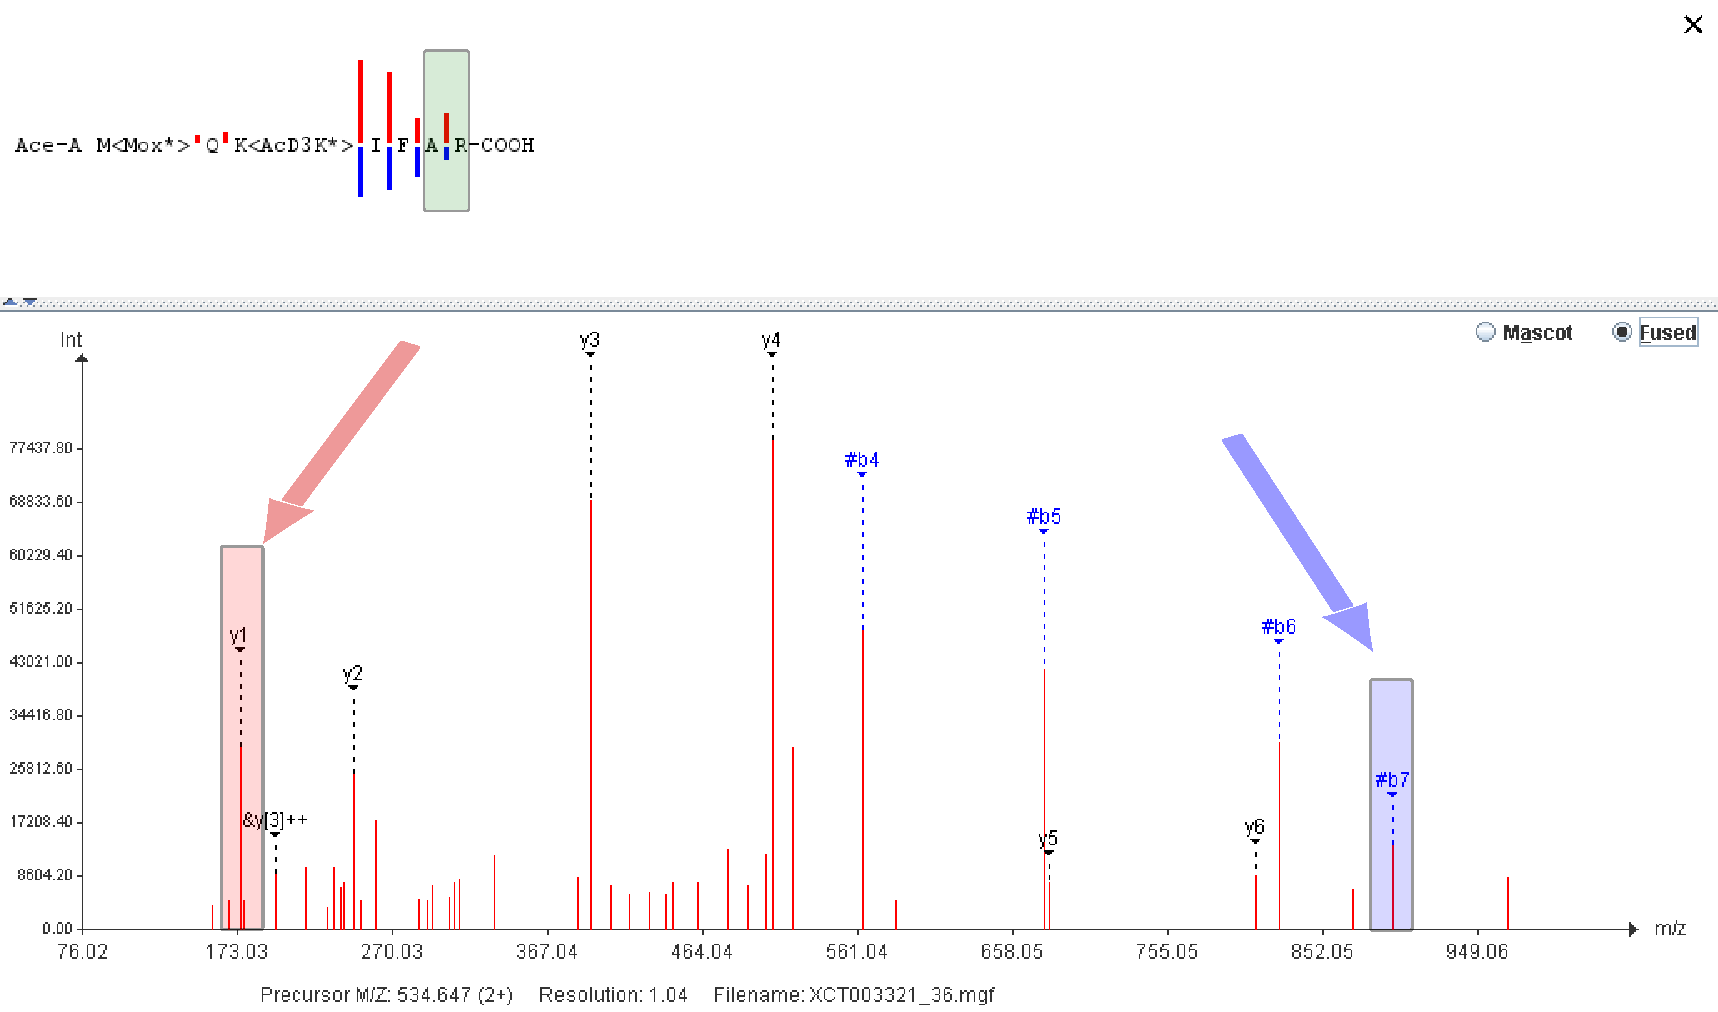
\includegraphics[width=.85\textwidth]{annotated_combining}
	\caption{\label{annotated_combining}The annotation on the peptide sequence in the top and on the MS/MS spectrum in the bottom are complementary. While the peptide sequence annotation is based on peptide bonds, the MS/MS spectrum annotation is based on mass over charge values.}
\end{center}
\end{figure}
%

\subsubsection{\label{information_table}General and Pluggable information}
\npar The bottom of the MS/MS spectrum identification tab contains an information-rich table on all confident peptide hypothesises. Both general and pluggable information are combined in this table.\npar An example is shown in figure \ref{table_main}.
%
%%%%%%
%FIGURE%
%%%%%%
\begin{figure}[h!]
\begin{center}
	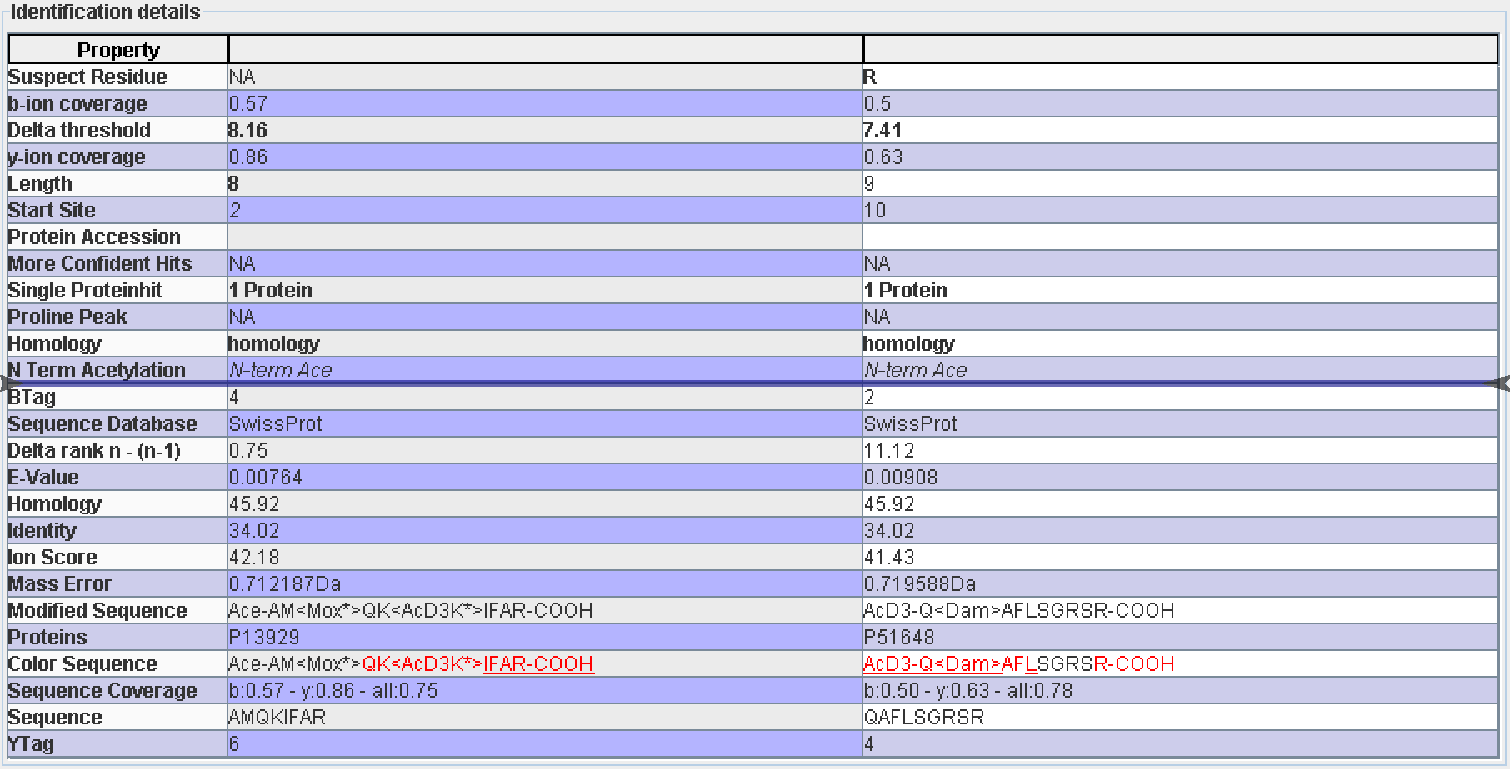
\includegraphics[width=.85\textwidth]{table_main}
	\caption{\label{table_main}The information table with both general and pluggable information. Each column shows a confident peptide hypothesis, ordered according to decreasing confidence from left to right. Each row shows an information unit. The upper rows show pluggable information driven by Agent inspections and the lower rows show general information. The Agent vote is reflected by the typeface of the cell.}
\end{center}
\end{figure}
%
\npar The first column lists the row identifiers. The other columns represent a confident peptide hypothesis, ordered according to decreasing confidence from left to right. By default, the most confident peptide hypothesis is focused by Peptizer. If there is more then one confident peptide hypothesis, right-click to select the appropriate column to focus on. The selected peptide hypothesis annotates the MS/MS spectrum and the sequence image. Moreover, by accepting a peptide hypothesis during validation, it is the focussed peptide hypothesis that is selected while the other peptide hypothesises, if any, are automatically rejected.
\npar The upper rows show pluggable information driven by Agent inspections. These cells display a peptide hypothesis property that was judged by the Agent. The cell's typeface also reflects the Agent vote.
\begin{description}
	\item[plain] when the Agent voted neutral for selection of the peptide hypothesis.
	\item[\textbf{bold}] when the Agent voted to select the peptide hypothesis.
	\item[\textit{italics}] when the Agent voted \textit{not} to select the peptide hypothesis.
\end{description}
%
\npar As such, one look at the table directly shows why Peptizer selected a peptide hypothesis.
\npar The lower rows show general information, which is always available. Examples are the peptide sequence, the protein source, the mass error, the MIS and the b-ion coverage.
%
\begin{center}
	\fbox{
        	 \begin{minipage}[t]{1.0\textwidth}
	            \textsc{Hint}\\A short tooltip describing the table row is shown by \textit{holding} the mouse above the row.
        	 \end{minipage}
             }
\end{center}
%
\npar Finally, the information table serves as a dense information scope on the peptide hypothesis. This complements the fragmentation information of the peptide hypothesis. As such, Peptizer provides an optimal environment to make the final decision on the validity of the peptide hypothesis proposed for a MS/MS spectrum.
\subsubsection{Validation}
\npar After a peptide hypothesis has been inspected by Agents and by the user, the user either rejects or accepts the peptide hypothesis.
\npar The validation functions are located in the right bottom part. To accept the peptide hypothesis, \textit{click }the button with the green OK icon. To reject the peptide hypothesis, \textit{click} the button with the red cross icon. Note that if there are multiple confident peptide hypothesises in the table, it is the focused peptide hypothesis that is validated. Also, if one is accepted, the others are automatically rejected. Both buttons (accept or reject) have an alternative button with an extra "text" mark. These buttons additionally show a dialog wherein the validation can be argued. If the validation status must be reset, click the button with the black reset sign. After validating a peptide hypothesis, its MS/MS spectrum identification tab will close before the next non-validated MS/MS spectrum identification tab opens.
\subsection{Status pane}
\npar The status pane is always available. Simple messages are logged in the top status panel while error messages are logged in the error window. 
%
%SAVE
%
\section{Saving the results}
\npar The input of Peptizer consists of MS/MS spectra and their peptide hypothesises. Within Peptizer these can be inspected by multiple Agents resulting in a custom selection of MS/MS spectra, which can then be validated. Then, the output of Peptizer consists of the same MS/MS spectra and their peptide hypothesises, however these are now labelled by Agent inspections and user validation. This additional information can be saved as well. Either in a comma separated file format or in an ms\_lims database.
\npar Save a selection task by by pressing \verb!Ctrl-S! or by \textit{clicking }the menu bar in the top:
% 
\begin{center}
\textit{Main // Save}	
\end{center}
%
\npar The save dialog has two main parts. The upper serves to select \textbf{which task} must be saved while the lower part serves to define \textbf{what information} must be included for each peptide hypothesis.
\subsubsection{Saving to comma separated value file}
\label{save_csv_txt}
Both the general and pluggable information shown in the table (see \ref{information_table}) can be written into a csv file. The save to csv dialog is shown in figure \ref{save_csv}.
%
%
%%%%%%
%FIGURE%
%%%%%%
\begin{figure}[H]
\begin{center}
	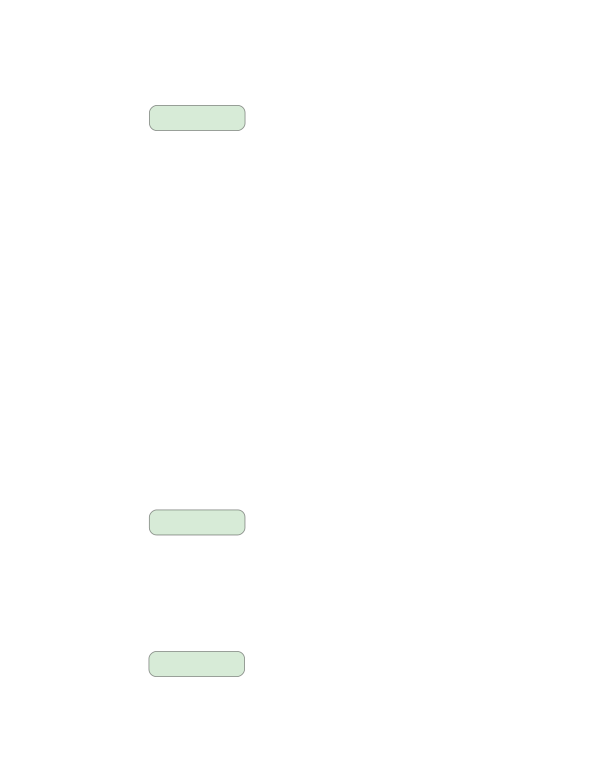
\includegraphics[width=.85\textwidth]{save_csv}
	\caption{\label{save_csv}This dialog window serves to save the output into a csv file. Define the desired \textbf{content} of the csv file by \textit{clicking} the check box aside an information cell. Below this content \textbf{options} to include other MS/MS spectra and their peptide hypothesis beside those selected by Peptizer are provided. Another kind of optional output are the user's validation comments. Finally, a \textbf{target} to save the csv file must be selected.}
\end{center}
\end{figure}
%
%
\npar In this window, the user can choose the content of the csv file. Three parts can be distinguished:
%
\begin{description}
	\item[Content]. Select the information that must be saved. This table mirrors the information table, so some or all of the general of pluggable information can be included in the comma separated file. 
	\item[Options].\\
	\begin{description} 
		\item[\textit{Include validation comments}] Add the user validation comments as the last column.
		\item[\textit{Include confident identifications that did not match the profile}] Add confident peptide hypothesises that were not selected by Peptizer.
		\item[\textit{Include non-confident identifications}] Add non-confident peptide hypothesises.
		\item[\textit{Include non-primary ranked hits}] Add all confident peptide hypothesises, also if they are ranked second or third.
	\end{description}
	\item[Target]. Select a target file to write the output to.
\end{description}
%
%
\subsubsection{Saving to PDF file}
\npar Where tab delimited files can be a starting point for further data analysis,  PDF files are definitely and end point. They have a single purpose for fast data sharing and therefore still useful as email communication or web sharing. The biggest advantage of PDF files being a wide spread format and high resolution graphics. \textit{Hence, sharing proteomics data in public repositories such as PRIDE or PeptideAtlas should be favored at all time!}
%
%%%%%%
%FIGURE%
%%%%%%
\begin{figure}[H]
\begin{center}
	
\includegraphics[width=.85\textwidth]{save_pdf}
	\caption{\label{save_pdf}The save method for a peptideidentification in PDF format. If there were multiple peptide identifications selected by Peptizer, then a single pdf file with multiple pages is created. }
\end{center}
\end{figure}
%
%
\subsubsection{Saving to ms\_lims database}
\npar If the ms\_lims database was used as data source, the user validation can be persisted into ms\_lims. The "save to ms\_lims" dialog is shown in figure \ref{save_ms_lims}. At this stage, the new information concerns the user validation. Therefore, no further options are provided as all the MS/MS spectra and their peptide hypothesises are already stored in the ms\_lims system.
%
%
\section{Distributing Peptizer objects}
\npar Selected peptide hypothesises in Peptizer stand over time and space. If 250 peptide MS/MS spectra and hypothesises must be manually validated, this could last a few days. Moreover, if doubts arise on validating a peptide hypothesis, a second opinion should be required. For this use case, Peptizer can store and load the content of the manual validation environment.
\npar Store a task by \textit{clicking }the menu bar in the top:
%
\begin{center}
\textit{Task // Store}	
\end{center}
%
%
\begin{description}
	\item[All] stores all the MS/MS spectra.
	\item[Accepted] stores the MS/MS spectra that have been accepted upon validation. (\textit{Those that are coloured green in the tree!})
\end{description}
%
\npar Load a task by \textit{clicking }the menu bar in the top:
%
\begin{center}
\textit{Task // Load}	
\end{center}
%
\npar Now, browse to the file that was previously stored to reload its content into Peptizer.
%
\begin{center}
	\fbox{
        	 \begin{minipage}[t]{1.0\textwidth}
	            \textsc{Hint}\\Go the example page on the Peptizer project web page to find such a file with a set of MS/MS spectra and validated peptide hypothesises that can be reloaded into Peptizer. This serves as an example set to start using Peptizer!\\(\url{http://genesis.ugent.be/peptizer/peptizer/download/examples.html})
        	 \end{minipage}
             }
\end{center}
%
\section{Understanding the configuration files}
\label{configuration_files}
\npar The configuration files are essential to the plug-and-play concept of Peptizer. When Peptizer starts, these configuration files declare which Agents and AgentAggregators are available to the user in Peptizer. Thus, when custom Agents are written in Java and added to the configuration files, they will function rightaway in the Peptizer platform.
\npar The configuration files are simple XML files and, as such, both computers and humans can easily read and modify them. They must reside in the same folder as the Peptizer start-up file. In total, there are four configuration files:
%
\begin{description}
	\item[agent.xml] lists the Agents that will be available to construct a voting panel and inspect peptide hypothesises.
	\item[aggregator.xml] lists the AgentAggregators that will be available to aggregate the Agent inspections.
	\item[table.xml] lists the general table rows that show the information in the information table.
	\item[general.xml] lists general configuration properties.
\end{description}
%
\npar Each of these are explained in the following subsections. 
\subsubsection{agent.xml}
\subsubsection{aggregator.xml}
\subsubsection{table.xml}
\npar All of these have a similar code structure. This is illustrated below by a section of the default agent.xml file.
%
\begin{verbatim}
<agent>
  1)  <!-- This Agent inspects the score delta between the MIS and MIT." -->
  2)  <uniqueid>be.proteomics.mat.util.agents.DeltaScore</uniqueid>
  3)  <property name="name">Delta threshold</property>
  4)  <property name="active">true</property>
  5)  <property name="veto">false</property>
  6)  <property name="delta">10</property>
</agent>
\end{verbatim}
%
\npar The outer \verb!<agent>! tags declare the start of a \textbf{new section}. This can also be aggregator or tablerow in the aggregator.xml or table.xml file respectively. Within this section, the following lines are present:
\renewcommand{\labelenumi}{\textbf{line \arabic{enumi}}.}
\begin{enumerate}
\item \textbf{describes} this section in a xml comment line. Note that this is only used as a guidance. The tooltip descriptions within Peptizer are hard coded.
\item \textbf{identifies} this section in a unique manner. Since Java guarantees that each class has a unique class name, this is used as the unique identifier for an Agent.\footnote{The class name consists of the package structure and ends with the class itself. Consider it as a road to the class file whereas the track starts from "be" to "proteomics" andsoon.}
\item \textbf{names} this section. It is the functional name used within the Peptizer GUI.
%
\renewcommand{\labelenumi}{\textbf{line \arabic{enumi}56}.}
%
\item \textbf{define custom properties} for this section. Both the active and veto must have default boolean values when Peptizer starts. Moreover, the delta parameters defines the delta value (here as the required score difference between MIS and MIT) upon that Agents inspection.
\end{enumerate}
\npar Note that if there are no options for an Agent, AgentAggregator or Tablerow, no custom property lines will be shown. Else, if there are multiple options, there will also be multiple custom parameter lines.
%%
%
%
\subsubsection{general.xml}
\npar These are various settings for the Peptizer application. Just like the other configuration files, the values can be modified by default Peptizer values.
%
\begin{verbatim}
<general>
	<!-- Default annotation radiobutton. -->
	<property name="RDB_ANNOTATION">0</property>
	<!-- Default tree height. -->
	<property name="TREE_HEIGHT">20</property>
	<!-- Default confidence throughout MAT. -->
	<property name="DEFAULT_ALPHA">0.05</property>
		. . . 
</general>
\end{verbatim}
%
\npar The outer \verb!<general>! tags line up the start of the \textbf{general properties part}.
\begin{description}
\item[RDB\_ANNOTATION] Set the default MS/MS spectrum annotation type for the GUI: 0 will show the Mascot annotations and 1 will show the Fused annotations (see \ref{annotationtypes}).
\item[TREE\_HEIGHT] Set the number of pixels between the tree nodes.
\item[DEFAULT\_ALPHA] Set the alpha value for starting a new selection task.
\item[ITERATOR\_FOLDER\_PATH] Set the preset folder for the Datfile folder data source. 
\item[ITERATOR\_FILE\_PATH] Set the preset file for the Datfile data source.
\item[SAVEVALIDATION\_CSV] Set the preset file for the Datfile data source
\item[MODIFIEDSEQUENCE\_FRAGMENTATION\_PANEL] Set the annotations on the modified or the non-modified peptide sequence if respectively true or false.
\item[CONNECTION\_PROPERTIES] Set the coordinates to establish a ms\_lims database connection. This file can include the DRIVER and URL fields from the connection dialog
		if Peptizer is used to connect to the ms\_lims database system.
\item[FUSED\_INTENSITY\_PERCENTAGE] Set the lower intensity threshold as a percentage in relation to the most intense fragmention up to where peaks from the MS/MS spectrum will be annotated.
\item[ENABLE\_CONFIDENT\_NONSELECTED\_OBJECT.OUTPUTSTREAM] Set Peptizer to stream confident peptide hypothesises that were not selected into a temporary file. If set to true, an extra option appears in the SavetoCSV function to save these peptide hypothesises as well. Note that this temporary file is deleted after Peptizer is closed and this comes along with a performance cost.
\item[ENABLE\_NONCONFIDENT\_OBJECT.OUTPUTSTREAM]  Set Peptizer to stream non-confident peptide hypothesises into a temporary file. As such, data on the negative population can easily be gathered. If set to true, an extra option appears in the SavetoCSV function to save these peptide hypothesises as well. Note that this temporary file is deleted after Peptizer is closed and this comes along with a performance cost. \npar Saving these allows to easily gather on the negative population of peptide hypothesises.
\end{description}
%
\section{Using Peptizer from the command line}
\npar Basically, this means that a new Peptizer selection task can be started by a single command. Commands are run from the commands window or from the shell respectively in a windows or a UNIX environment. As this is no convenient environment for most users, running Peptizer from the command line should only be considered by informatics oriented users.
\npar Why is this useful? By the command line, multiple Peptizer tasks can be started with each task having a different Agent configuration or a distinct data source. Also, a Peptizer selection task can be started at a central server without any graphical interaction.
\npar This can be done in three steps:
\renewcommand{\labelenumi}{\textbf{\arabic{enumi}}.}
\begin{enumerate}
\item \textbf{Sets the classpath} to define the classes that must be loaded into the Java virtual machine.\footnote{Find out more on the Java classpath at \url{http://java.sun.com/j2se/1.3/docs/tooldocs/win32/classpath.html}} Therefore, this part defines the libraries required by Peptizer.\footnote{The Java libraries required by Peptizer are listed at the project website download page \url{http://genesis.ugent.be/peptizer/peptizer/download/main.html}}\\\verb!set CLASSPATH=.\config;.\peptizer-1.1.jar;.\mascot_datfile-1.5.3.jar; ..!
\item \textbf{Starts a Java process} by a command. Note that here you can also supply Java Virtual Machine properties as a parameter. In the example, \verb!-Xmx512M! reserves 512mb of memory to run this Peptizer task. Finally in this step, the Peptizer Class is supplied whose main method can start a Peptizer task in command line mode.
\\\texttt{java -Xmx512m be.proteomics.mat.main.Peptizer}
\\
\item \textbf{Sets the program parameters} to run a selection task.
\begin{verbatim}
--sourcetype file
--source C:\\Temp\\F004071.dat
--target C:\\Output\\result.csv
--table C:\\applications\\Peptizer\\table.xml
--agent C:\\applications\\Peptizer\\agent.xml
--aggregator C:\\applications\\Peptizer\\aggregator.xml
--general C:\\applications\\Peptizer\\general.xml
--parsing memory

\end{verbatim}
\end{enumerate}
\npar Note that by running \texttt{be.proteomics.mat.main.Peptizer} without the program parameters a help text appears in the command line.
\npar This will select all confident peptide hypothesises from \verb!F004071.dat! that match the profile by the Agents and AgentAggregator defined in \verb!agent.xml! and \verb!aggregator.xml!. The probability of a confident peptide hypothesis is defined in \verb!general.xml!. Finally, a csv file will be written as \verb!result.csv! containing general, pluggable information and a selection label as columns.
